
\section{Results}
\subsection{Demonstrating Features of the Method}

To get a sense of the accuracy of our novel approach to estimating multivariate effects, we simulated two types of data: shared, and tissue specific.



 In both settings, in which we expect our method to be superior to both univariate methods and joint methods in which the configuration approach is utilized, we simulate 50,000 gene-snp pairs, with only 400 representing true signal. This represents roughly 500 genes with 100 snps in cis, $80\%$ of which contain one active QTL. Thus naturally, if the gene contains such a QTL, it is the same QTL among all tissues in which the tissue is active. This puts a dual burden on the ability of the method to accurately capture effect sizes and shapes: the small number of true associations present in these simulations tests whether the method accurately encourages small observed effects toward zero while preserving the true signal when it exists. Furthermore, the  multivariate nature of these simulated `true' effects tests the ability of the method to accurately infer patterns of sharing from the dataset. These 400 true effects are thus simulated from the `learned' covariance matrices representing $U_{k}$ 2-9 in the GTeX dataset according to (\ref{eqn:mixprior}) and thus aim to emulate the patterns of sharing present in real biological data. We then simulate vectors of observed $\bm{\hat{\beta_{j}}}$ and their corresponding $\bm{Z_{j}}$ for all 50,000 gene-snp pairs (the majority of which represent `noise') according to (\ref{eqn:new_lik}) (see Methods \ref{sssec:simulation}) for details. %we simply simulate a vector of Error ($\textbf{E}_{j} \sim {\it N} (.; \bm{0}, V_{j} )$ where $V_{j} $ represents the diagonalized matrix of squared known standard error, $\bm{s}_{j}^{2}$) and then $\hat{\bm{b}}_{j} | \bm{b}_{j} , V_{j} = \bm{b}_{j} + \textbf{E}_{j}$ (see \label{sssec:simulation}). 
 We call this the `sharing' (S) scenario. 

 We compare with univariate `shrinkage' method Ash (Stephens et al, unpublished) as well as a modified version of eqtlBMA-lite (Flutre et al, 2013), here deemed `mash-lite' which uses the singleton and fully consistent (i.e., active in only one tissue, or active with the same effect size in all tissues) configurations to estimate these effects jointly (see Methods \ref{sssec:num1} item 6 for details).  
 One might expect that our method would prove superior only in the setting in which true effects are shared among all tissues, and thus fail in the setting of tissue specificity. Thus, building on the situation above, we add a simulation in which $35\%$ of the true effects are active in only one tissue, according to 5 different patterns of tissue specificity. We call this the `tissue-specific' (TS) scenario. 

We see that in terms of both power and accuracy, Matrix Ash, here deemed 'MASH' is superior in each simulation setting, to both univariate methods and to existing joint analysis approaches (mash-lite).
\begin{equation}
RMSE = \sqrt(\sum_{jr}(b_{jr}-E(b_{jr}|Data)^2))
\end{equation}
\begin{table}[ht]
\caption{Accuracy Comparison: RMSE}
\centering
\begin{tabular}{c c c c}
\hline\hline
Inference Method & MASH & ASH & mash-lite \\ [0.5ex] % inserts table %heading
\hline
RMSE_{S}&0.010&0.030&0.047\\
RMSE_{TS}&0.008& 0.025&0.043\\ %cor.with.truth_{S}&0.99&0.94&0.84\\
%cor.with.truth_{TS}&0.99&0.94&0.82\\
\hline
\end{tabular}
\label{table:RMSE}
\caption{\textbf{Accuracy Analysis} Above we compare the ability of Matrix Ash (`MASH') to capture the true effect size estimates. We compare with univariate-shrinkage method `ASH' and configuration-specific joint approach `mash-lite'. We report the Root Mean Squared Error (RMSE) and the correlation with the truth.}
\end{table}

To demonstrate the ability of MASH to powerfully capture these accurately estimated effect sizes, we compare the proportion of true associations called significant at a given significance threshold among the three methods. Indeed, MASH proves superior to both methods under each condition (i.e., sharing or tissue-specific).

\begin{figure}[h]
\includegraphics[width=5cm]{Figures/PlotsForPaper_files/figure-html/unnamed-chunk-5-1.png}&
\includegraphics[width=5cm]{Figures/PlotsForPaper_files/figure-html/unnamed-chunk-5-2.png}
\caption{\textbf{Power vs Accuracy} \textbf{Left}: Under both the Shared (not shown) and Tissue Specific settings, we identify a greater number of true associations at a given local false sign rate threshold using MASH then either univariate methods (ASH) or joint `configuration style' approaches (mash-lite). \textbf{Right}: Similarly, among associations we deem to be calling correctly at various thresholds, we are able to correctly identify the sign of the effect in many more instances using MASH then either univariate methods (ASH) or joint `configuration style' approaches (mash-lite).}
\label{fig:powervaccuracy}
\end{figure}\newline

In introducing a method to quantify the heterogeneity of effect sizes, we have developed a `heterogeneity index' which attempts to capture the heterogeneity in magnitude among tissues in which the gene-SNP pair is active. For each gene-snp pair $j$, we normalize its vector of effects $\bm{b_{j}}$ across tissues by the effect which has the maximum absolute value; thus for a fully `consistent' gene-snp pair in which all the effects are equal in magnitude, the new vector of normalized effects would consist of all ones, and R=44 tissues would be greater than $50\%$ of the maximum effect. By contrast, for a tissue-specific gene-snp pair, the vast majority of effects would be small fraction of the maximum effect and thus the number of tissues greater than $50\%$ of the maximum effect would be 1 (the effect used to normalize). We can apply this heterogeneity index, here deemed $\textbf{`HI'}$ to the real data, but first wanted to demonstrate the superiority of MASH in estimating these quantities on simulated data. To quantity the ability of each method to accurately ascertain the heterogeneity, we can compute the heterogeneity index of the real data, and the inferred quantities, and use a modified RMSE:

\begin{equation}
RMSE_{HI} \sqrt(\sum(true_{HI}-estimated_{HI})^2)
\end{equation}

\begin{table}[ht]
\caption{Accuracy Comparison: RMSE}
\centering
\begin{tabular}{c c c c}
\hline\hline
Inference Method & MASH & ASH & mash-lite \\ [0.5ex] % inserts table %heading
\hline
HI_{S}&39.38 &40.87 &39.78 \\
HI_{TS}& 39.98& 40.77&39.51\\
\hline
\end{tabular}
\label{table:HETindex}
\end{table}

\subsubsection{Adaptive Shrinkage: The Multivariate Approach}

To demonstrate the utility of shrinking effect size estimates jointly, we consider the estimated effect sizes against their observed input summary statistics using our joint (MASH) and comparing to a univariate shrinkage method (Ash). On simulated data, we can also then plot the estimated effect sizes against the true values, again comparing among methods. Here, we show the results under the setting of tissue specificity, to analyze the behavior of eQTL of each class.

%\textbf{Figure: Insert Simulations from TSpecific Conditions here}
\begin{figure}[htbp]
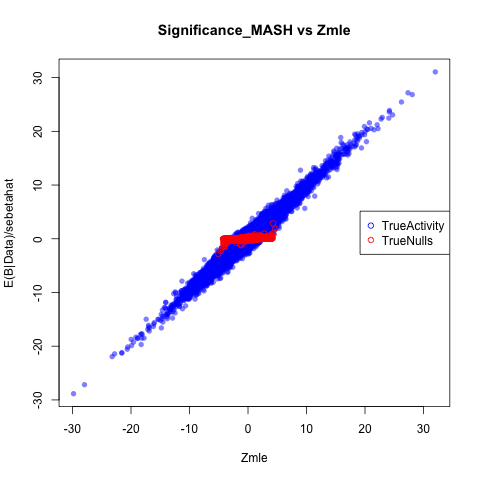
\includegraphics[width=5cm]{Figures/scatterplot_fittedtspec.png}&
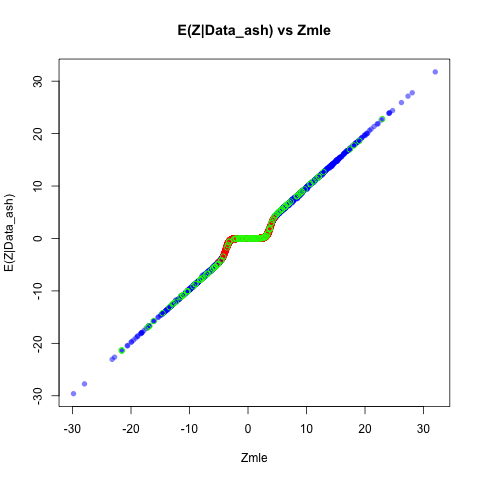
\includegraphics[width=5cm]{Figures/scatterplot_fittedtspec_ash.png}\\
%\hfill
%%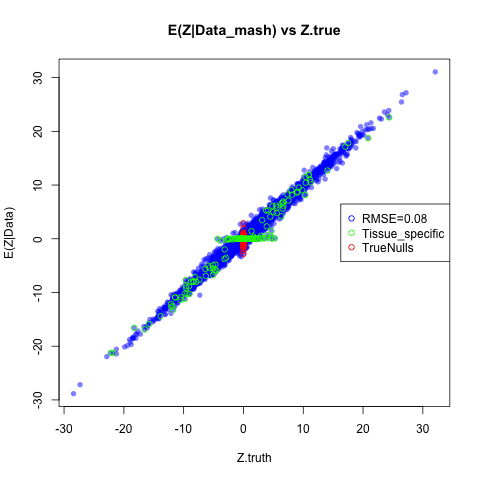
\includegraphics[width=5cm]{Figures/scatterplot_truthtspec.png}&
%%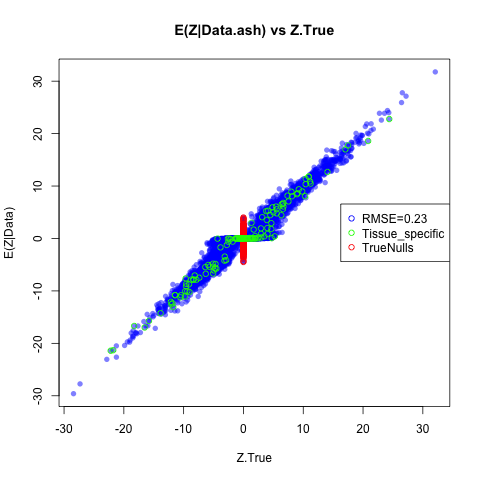
\includegraphics[width=5cm]{Figures/scatterplot_TRUTHashtspec.png}
%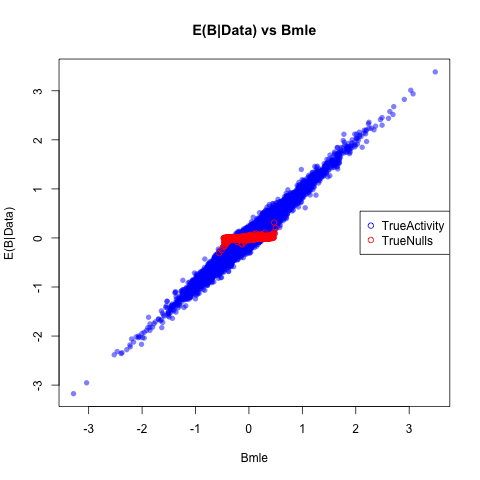
\includegraphics[width=5cm]{Figures/scatterplotfittedbspec.png}&
%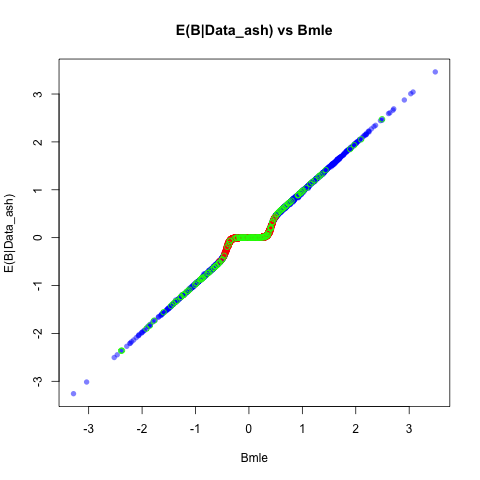
\includegraphics[width=5cm]{Figures/scatterplotfitted_bspec_ash.png}\\
%\hfill
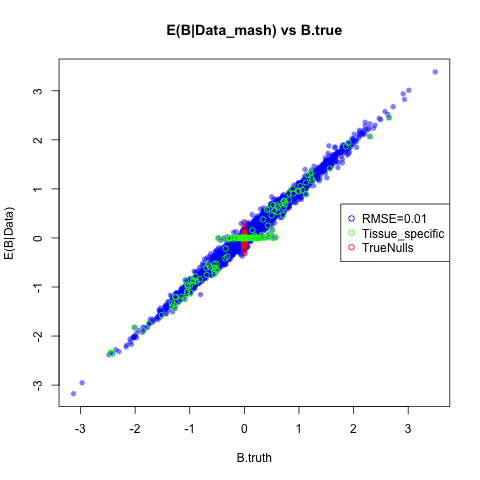
\includegraphics[width=5cm]{Figures/scatterplot_truthbspec.png}&
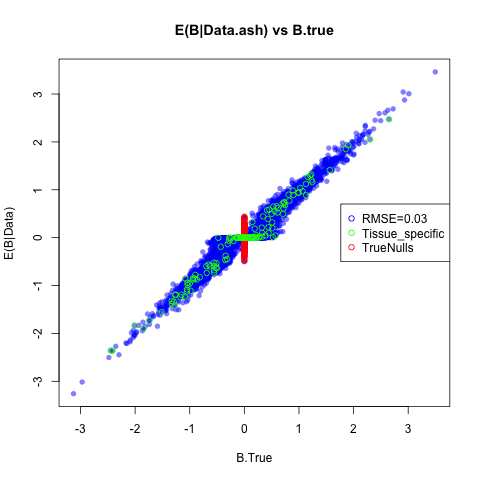
\includegraphics[width=5cm]{Figures/scatterplot_TRUTHashbspec.png}
\caption{\textbf{Understanding Power and Accuracy Gains}: \textbf{Top Left}: We contrast the power advantage of a joint shrinkage approach with that of a univariate thresholding approach, in which all observed statistics of a given level of significance shrunk equivalently, independent of the information contained in other tissues. Using the information contained in other tissues allows us to augment (or shrink less harshly) small effects in one tissue in the presence of evidence of strong effects in other tissues, while univariate methods ignore alternative tissues. Thus the method is dually `adaptive' by considering the abundance of both effect sizes (here, an abundance of small effects) and shapes in the overall data-set. $\textbf{Bottom}$: the correlation with the true (simulated) effect sizes values is greater using MASH (left) then univariate methods (right), and truly null values are shrunk more harshly, while retaining the ability to capture tissue-specific eQTL.}
 \label{fig:simulationscatter}
\end{figure}\newline
%
%In both MASH and univariate methods, $\hat{b}_{jr}$ of a given size will be shrunk more harshly depending on their errors (Ash Paper, Stephens $\emph{et al}$). 
%%However, under the `EZ' model used here, the standard errors are uniformly one, and thus effects are shrunk according to the ratio between their observed effect $\hat{b}_{jr}$  and their standard error $\hat{s}_{jr}$. 
%However, plotting the estimated significance (i.e., $\frac{E(B|Data)}{\hat{s}_{j}}$) against the observed Z score (i.e., $\hat{Z}_{jr})$ (Figure \ref{fig:simulationscatter}) allows us to understand the behavior of multivariate versus univariate methods once the standard error has been considered. 
In a univariate method, all effects with the same observed effect size $\hat{b}_{jr}$ and standard error $\hat{s}_{jr}$ and accordingly the same Z statistic will be shrunk equivalently, while a joint method allows us to consider effects in other tissues in augmenting the posterior estimated effect size and its corresponding estimate of significance.
%However under the simulation framework here, where the standard errors are roughly uniform across tissues, plotting estimated efect sizes (i.e., $E(b_{jr}|Data$)) against the observed `raw' input values (i.e., $\hat{b}_{jr})$ (Figure \ref{fig:simulationscatter}) allows us to understand the behavior of multivariate versus univariate methods once the standard error has been considered. 
In this simulated data-set, where there is an abundance of small effects, both univariate and multivariate methods tend to shrink small observed values of $\hat{\bm{b}}$ towards prior mean at $\bm{0}$ as their likelihoods will be maximized by component with small $\omega$. However, while univariate methods shrink all observed Z statistics uniformly, thus preserving their rank-order of significance, MASH does not. Critically, this is due to the power of joint analysis to consider the effects across tissues in inferring the final vector of effect sizes, and allowing evidence contained in all tissues jointly to augment our posterior estimate of significance. Thus the method is dually `adaptive' by considering the abundance of both effect sizes and shapes in the overall data-set.  Here, acknowledging consistency, small effects in one tissue will be augmented in the presence of larger effects in other tissues, resulting in dramatic power increases (Figure \ref{fig:powervaccuracy}).

Furthermore, when we plot the estimated effects $E(\beta_{jr}|Data)$ against true effect size $\beta_{jr}$ (Figure \ref{fig:simulationscatter}, $\textbf{bottom}$) and segregate these effects by class  (e.g., active and shared, active and tissue-specific, or null), we see that the correlation among the true and estimated effect $E(\beta|D)$ sizes is much tighter using our multivariate approach. Similarly, truly null effects are shrunk more tightly, due to the fact that in the presence of consistency, small effects across subgroups will lead us to have a high prior belief that an additional small observed effect in that eQTL is also likely to be close to 0. Importantly, tissue-specific QTLs are still captured using our joint approach, demonstrating that if tissue-specific patterns exist in the data, our prior belief will capture this phenomenon and accordingly our posterior estimates will reflect the underlying tissue-specific nature at a given tissue-specific SNP.

Together, these results demonstrate the tremendous power increase of using a multivariate method and the accuracy of estimating patterns of sharing from the data rather than imposing forced configurations which fail to capture the heterogeneity of effect sizes among tissues.


\subsubsection{Power and Adaptive Shrinkage: Real Data}

Now, we consider the results of our analysis, when applied to the GTEX data set. After estimating the covariance matrices from the strongest gene-snp pairs, in an effort to capture the underlying 'true patterns' of sharing in the data and adding the qualitatively specific configurations `mash-lite' configurations, we can infer the relative frequency of each pattern of sharing and corresponding effect sizes from a large sample of 40,000 gene-snp pairs (see Methods for details on prior weight estimation).

Here, we report the analysis on the top SNP for each of 16,069 genes, where the `top' snp is defined as the SNP with the largest observed univariate Z-statistic in absolute value across tissues. As described above and demonstrated in simulations, in the setting of an abundance of small effects in data set, MASH tends to shrink small observed values towards the prior mean at $\bm{0}$. It should be noted that this is a result specific to a particular data set, and in that sense `adaptive' - indeed, if small effects were rare and large effects abundant, such shrinkage would not occur. 

But perhaps more importantly, there is a striking increase in power (Table \ref{table:power}) when compared to univariate methods. There are a total of 44 tissues x 16,069 gene-snp pair associations considered, or 707,036 total tissue-level effect size coefficients. At an $lfsr$ threshold of 0.05, we identify 393,414 significant snp-gene-tissue effects ($b_{jr}$). Using estimates shrunk according to a univariate approach (again, Ash),  we identify only 91,755, meaning that using univariate methods we would be confident our ability to identify the sign in only $13\%$ of cases, while using our joint procedure for estimating effects, we would confidently argue the SNP has a non-zero effect for a gene in a particular tissue over half $(55\%)$ of the time. As described, this tremendous increase in power arises from the fact that in the presence of  a data set possessing consistency, as learned by the hierarchical model, small effects in the presence of a gene containing large effects in alternative tissues will be augmented to reflect such consistency, thus increasing our confidence in its size and direction. While the number of associations capture is slightly greater using the mash-lite approach, we note that the likelihood of the data set under this model is much much worse ($-1298672$ vs $-1267997.5$, see supplementary data `Testing and Training' procedure). Critically, `mash-lite' would put the vast majority of the prior weight on the fully `consistent' configuration (Figure \ref{fig:pihat}), as SNPs demonstrating activity across all tissues, regardless of how heterogeneous among subgroups, are forced into this configuration. Simulations above demonstrate the lack of accuracy arising from such an approach.%\newline


%\textbf{Figure: Real Data Scatterplot}
\begin{figure}[htbp]
%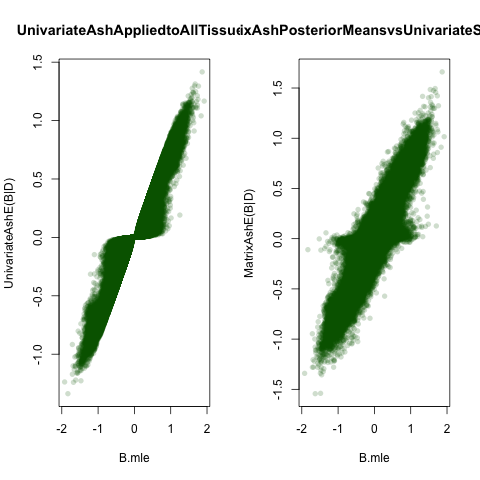
\includegraphics[width=5cm]{Figures/comparebeta.png}&
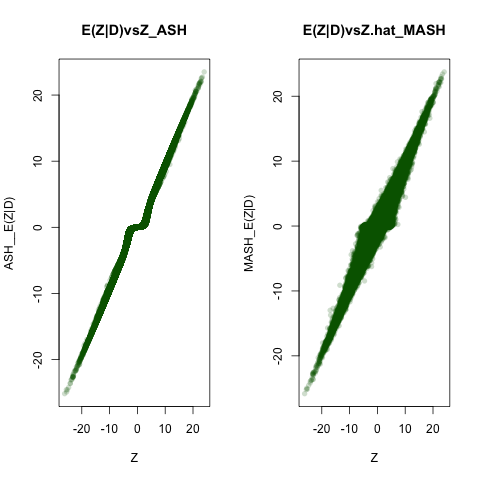
\includegraphics[width=10cm]{Figures/comparez.png}\\
%\caption{\textbf{Understanding Shrinkage with Real Data} While both univariate and joint methods shrink estimates $\hat{b_{jr}}$  of a given size with large standard error more harshly ($\textbf{Left two panels)}$, comparing the posterior estimates for a given observed $Z$ statistic ($\textbf{right two panels)}$ allows us to visualize the power of joint analysis. Since all observed $Z$ statistics have a standard error of one, 
\caption{\textbf{Power of Joint Analysis in Real Data} From real data: Z statistics of the same size are shrunk differently depending on the effect across tissues using our joint approach MASH ($\textbf{right}$), when compared to univariate methods $\textbf{left}$, which tend to shrink all observed effects of a given size and standard error (i.e., equivalent Z statistics) uniformly, resulting in tremendous power gains (Table $\ref{table:power}$) by the increased significance induced.}
\end{figure}\newline

\begin{table}[ht]
\caption{Power Comparison}
\centering
\begin{tabular}{c c c c}
\hline\hline
Metric & LFSR_{MASH} & LFSR_{ASH}&mash-lite \\ [0.5ex] % inserts table %heading
\hline
Significant $\bf{b}_{jr}$ $\leq$ 0.05%&202087
&393,414 & 91,755&401,552\\
%$\bf{b}_{jr}$ significant in other not in MASH %&8649
%&NA&1447 \\
%$\bf{b}_{jr}$ significant in MASH not in other %&199976
%&NA&303106 \\[1ex]
\hline
\end{tabular}
\caption{\textbf{Power} Restricting our analysis to thresholding by local false sign rates, we can quantify the number of associations we identify at a given local false sign rate threshold using the original summary statistics and posterior means computed using multivariate MASH and Univariate Ash. We can see that MASH calls over four times as many associations significant when compared to univariate approach, and is comparable in power to a less-accurate joint approach (mash-lite)}
\label{table:power}
\end{table}\newline



%\textbf{Figure: $\hat{\pi}$ barplot in MASH vs BMAlite}
%\newline
\begin{figure}[htbp]
\includegraphics[width=10cm]{Figures/PlotsForPaper_files/figure-html/unnamed-chunk-9-1.png}
\caption{\textbf{Prior Weight Assigned to Patterns of Activity} While a joint method like `mash-lite' assigns the majority of the prior weight to the `consistent' (active across all tissues with the same prior effect size) configuration, we can see that MASH is able to accurately parse shared configurations, thus resolving the relationship among tissues in which the QTL is active. This is a superior model fit, as judged by the likelihood improvement and simulation results above.}
\label{fig:pihat}
\end{figure}\newline





\subsection{A qualitative description of heterogeneity in the GTEX data}

Indeed, from the prior weight assigned to the `learned matrices' (Figure \ref{fig:pihat}) coupled with the simulation results in the previous sections, we can see that MASH is able to accurately parse shared configurations, thus resolving the relationship among tissues in which the QTL is active Figure \ref{fig:pihat}, \ref{fig:pcplot} and Supplementary Figure \ref{fig:allheat}. 
%To further contrast our approach with existing joint methods on this data-set, consider a two-tissue example, in which a configuration type approach recognizes only patterns constrained to lie along the x and y axis or along the $x-y$ line (Figure \ref{fig:Patterns}). MASH allows for patterns which show consistently larger effects in one tissue over another, with varying amounts of correlation among tissues. In these examples from real data (Figure \ref{fig:twoplot}), we can see that while eQTL of the green, blue and yellow class appear consistently active in both Brain and Muscle , the blue and yellow effects have consistently larger effects in Skeletal Muscle than brain, while SNPs of the green class show the reverse. Similarly, eQTL of the yellow class show only loose correlation among this chosen pair of tissues, while eQTL of the blue class show strong correlation between this pair. Furthermore, we can see that eQTL of the pink class tend to show tissue-specificity in Whole Blood relative to testis, while eQTL of the black class show tissue specificity in testis relative to whole blood. Lastly, within QTL of the yellow class, there exists only loose correlation between testis and lymphocytes, but strong correlation among colonic tissues, indicating the value of capturing distinct patterns of correlation among different pairs of tissues among SNPs of a given class, or between classes. 
%%\newline
To emphasize the contrast  between our approach and existing joint methods on this data-set, we compare our results to a configuration approach which recognizes only patterns constrained to lie along the x and y axis or along the $x-y$ line (Figure \ref{fig:Patterns}). MASH allows for patterns which show consistently larger effects in one tissue over another, with varying amounts of correlation among tissues.   We compare the first principal component of each of these covariance matrices reflecting the patterns `learned' from the data and used as $U_{k}$ to model the effect size for each gene-snp pair $\bm{b}_{j}$ in $\ref{eqn:mixprior}$ (see Methods \ref{sssec:num1} for details). Intuitively, this provides a cursory approximation of the relationship in effect sizes among tissues (Figure \ref{fig:pcplot}) captured by each pattern. 

\begin{figure}[htbp]
\includegraphics[width=10cm]{Figures/PlotsForPaper_files/figure-html/unnamed-chunk-28-1.png}
\caption{\textbf{Relationships Among Tissues Captured} Here, we demonstrate the first principal direction of each pattern of effects across tissues, by simply taking the first eigenvector of each of these covariance matrices. Intuitively, these provide a rank 1 summary of the relationship in effect sizes and directions among tissues captured by each pattern. They can be contrasted with the `consistent configuration' which assumes the same effect size for all tissues in which the tissue is active. See Text for details and possible interpretations, and Supplement for guide to tissue abbreviations.}
\label{fig:pcplot}
\end{figure}\newline
%\textbf{Figure: Colored Scatterplots of 2 tissues, contrasting effects between tissues, color coded by responsibility}
%\newline

%\begin{figure}[htbp]
%\includegraphics[width=5cm]{Figures/PlotsForPaper_files/figure-html/unnamed-chunk-10-1.png}&
%\includegraphics[width=5cm]{Figures/PlotsForPaper_files/figure-html/unnamed-chunk-10-3.png}\\
%\hfill
%\includegraphics[width=5cm]{Figures/PlotsForPaper_files/figure-html/unnamed-chunk-10-4.png}&
%\includegraphics[width=5cm]{Figures/PlotsForPaper_files/figure-html/unnamed-chunk-10-5.png}
%\caption{\textbf {Diverse Array of Relationships among tissues.} While eQTL of the green, blue and yellow class appear consistently active in both Brain and Muscle, the blue and yellow effects have consistently larger effects in Skeletal Muscle than brain, while SNPs of the green class show the reverse. Similarly, eQTL of the yellow and blue class show weak and strong correlation among Muscle and Brain, respectively. Similarly, we can see that eQTL of the pink class tend to show tissue-specificity in Whole Blood relative to testis, while eQTL of the black class show tissue specificity in testis relative to whole blood. Lastly, QTL of the yellow class seem only loosely correlated between testis and lymphocytes, but strongly correlated among colonic tissues.}
%\label{fig:twoplot}
%\end{figure}
%

%
%\begin{figure}
%    \centering
%    \begin{subfigure}[b]{0.4\textwidth}
%        \includegraphics[width=5cm]{Figures/PlotsForPaper_files/figure-html/unnamed-chunk-10-1.png}
%        \caption{Testes vs Whole Blood}
%        \label{fig:testes}
%    \end{subfigure}
%    ~ %add desired spacing between images, e. g. ~, \quad, \qquad, \hfill etc. 
%      %(or a blank line to force the subfigure onto a new line)
%    \begin{subfigure}[b]{0.4\textwidth}
%        \includegraphics[width=5cm]{Figures/PlotsForPaper_files/figure-html/unnamed-chunk-10-3.png}
%        \caption{Muscle vs Brain}
%        \label{fig:musclevbrain}
%    \end{subfigure}
%%add desired spacing between images, e. g. ~, \quad, \qquad, \hfill etc. 
%    %(or a blank line to force the subfigure onto a new line)
% 
%    \begin{subfigure}[b]{0.4\textwidth}
%        \includegraphics[width=5cm]{Figures/PlotsForPaper_files/figure-html/unnamed-chunk-10-4.png}
%                \caption{Testes vs Lymphocytes}
%        \label{fig:testesvslymphocytes}
%    \end{subfigure}
%        ~ %add desired spacing between images, e. g. ~, \quad, \qquad, \hfill etc. 
%      %(or a blank line to force the subfigure onto a new line)
%    \begin{subfigure}[b]{0.4\textwidth}
%        \includegraphics[width=5cm]{Figures/PlotsForPaper_files/figure-html/unnamed-chunk-10-5.png}
%        \caption{Colon Sigmoid vs Tranverse}
%        \label{fig:colon}
%    \end{subfigure}
%    \caption{\textbf {Diverse Array of Relationships among tissues.} While eQTL of the green, blue and yellow class appear consistently active in both Brain and Muscle (\ref{fig:musclevbrain}) , the blue and yellow effects have consistently larger effects in Skeletal Muscle than Brain, while SNPs of the green class show the reverse. Similarly, eQTL of the yellow and blue class show weak and strong correlation among Muscle and Brain, respectively. Similarly, we can see that eQTL of the pink class tend to show tissue-specificity in Whole Blood relative to testis  (\ref{fig:testes}), while eQTL of the black class show tissue specificity in testis relative to whole blood. Lastly, QTL of the yellow class seem only loosely correlated between testis and lymphocytes (\ref{fig:testesvslymphocytes}), but strongly correlated among colonic tissues (\ref{fig:colon}).}
%\label{fig:twoplot}
%\end{figure}

Each of the $U_{k}$ thus reflects diverse relationships in effect sizes among tissues: for instance, comparing the black and red pattern, we see that gene-snp pairs with high posterior probability of arising from the black class ($U_{k}=2$) demonstrate consistently smaller and shared effects in brain than other tissues, while gene-snp pairs of the red class ($U_{k}=3$) demonstrate strong effects in brain as compared to alternative tissues, for example. Indeed, matrix $U_{k}$ = 3 captures gene-snp pairs with large, correlated effects in brain, and is the most prevalent pattern of sharing in the larger data set, as reflected by it's prior weight summed across effect size (see Figure \ref{fig:pihat}). Matrix $U_{k}$ = 2 captures SNPs with small effects in brain and larger effects in thyroid and transformed cell-types (e.g., fibroblasts, lymphocytes).
Similarly, we see that the patterns learned in $U_{k}$ =4, 5 and 8 (blue and yellow) demonstrate a degree of `quantitative' specificity: that is, consistently stronger effects in one tissue (whole blood, whole blood and testes, respectively) without restricting the effect sizes to zero in alternative tissues. Because these patterns and their relative abundance are `learned' from the data and allow for a superior model fit to methods which restrict effects as `active' or `qualitatively specific', we can use these to understand gross patterns present in the data as well as gene-snp specific effects. Examining the barplot (Figure \ref{fig:pihat}) of the relative importance of each of these patterns as learned from the data through empirical Bayes Methods (See methods \ref{sssec:ebweights}) and comparing it with a method which simply calls effects `active or inactive' (mash.lite) we see that such patterns are able to effectively `dissect' the activity quantified in a fully `consistent' configuration.

%
%For instance, learned matrix $U_{k}$ = 3 captures gene-snp pairs with large, correlated effects in brain, and is the most prevalent pattern of sharing in the larger data set, as reflected by it's prior weight summed across effect size (see Figure \ref{fig:pihat}). Matrix $U_{k}$ = 2 captures SNPs with small effects in brain and larger effects in thyroid and transformed cell-types (e.g., fibroblasts, lymphocytes). Several of the lower rank matrices whose patterns receive high prior weighting (e.g., $U_{k}$ = 4,5,8 and 9) show somewhat tissue specific (i.e., high prior variance in only one tissue-type) effects in testes and whole blood, consistent with our conclusions that whole blood and testes indeed demonstrate an abundance of tissue-specific gene-snp pairs. 



\subsubsection{Examples of Select Patterns}

Here we examine several example gene-snp pairs with a high posterior probability of arising from the covariance patterns captured by our model. We deem this posterior probability of arising from a particular pattern as a high `loading' or `responsibility.' We consider the posterior effect, as normalized by it's standard error, to see how the significance across tissue combines information contained in the prior pattern which the gene-snp pair most resembles, and the data originally observed.
%\newline
%\textbf{Figure: High loading on UK3: Captures correlation in sign, quantitative heterogeneity in magnitude along diagonal emphasizes the utility of continuous approach}
%\newline
\begin{figure}[htbp]
\includegraphics[width=6cm]{Figures/PlotsForPaper_files/figure-html/unnamed-chunk-12-1.png}&
\includegraphics[width=8cm]{Figures/PlotsForPaper_files/figure-html/unnamed-chunk-12-2.png}\\
\includegraphics[width=6cm]{Figures/PlotsForPaper_files/figure-html/unnamed-chunk-13-1.png}&
\includegraphics[width=8cm]{Figures/PlotsForPaper_files/figure-html/unnamed-chunk-13-2.png}\\
\includegraphics[width=6cm]{Figures/PlotsForPaper_files/figure-html/unnamed-chunk-14-1.png}&
\includegraphics[width=8cm]{Figures/PlotsForPaper_files/figure-html/unnamed-chunk-14-2.png}\\
\caption{\textbf{High loading on $U_{k}$=3, $U_{k}$=5, and mash-lite}:  While all matrices appear to capture overwhelming correlation in sign, the varying degrees of quantitative heterogeneity in magnitude along the diagonal emphasize the utility of continuous approach. The correlation in sign means that erratic `off-directions' in observed statistics are often flipped ($\textbf{top}$). $\textbf{Center}$: this gene snp-pair demonstrates high loading on the learned (as opposed to forced) pattern of activity $U_{k}=5$ which captures quantitatively specific activity in whole blood. Effects are significant in many tissues, but quantitatively specific to whole blood. $\textbf{Bottom}$: we also find evidence of qualitative heterogeneity, reflected in the example demonstrating high loading on mash-lite configuration matrix, and accordingly only the activity in whole blood is deemed significant.}
\label{fig:uk3}
\end{figure}


In this particular example (Figure \ref{fig:uk3}, top), with high posterior probability of arising from the pattern captured by $U_{k}=3$, strong, shared effects in brain tissues match an underlying pattern of shared effects present in the larger data set and thus allows this gene-snp pair to find its true match. Brain effect sizes thus borrow strength from one another, and accordingly, the posterior estimates tend to nudge the brains towards a consistent, shared effect. Similarly, an overall tendency towards consistency in sign in the larger data set, as captured by the hierarchical model and reflected in the positive correlation in sign among all tissues, tends to `flip' erratic off directions towards the prevailing positive direction. Heterogeneity in magnitude among the other tissues is reflected in the variety of banding intensity along the diagonal.\newline

%
%%\textbf{Figure: UK 9: Quantitative specificity in magnitude in Testes/Whole Blood}
%\newline
%\begin{figure}[htbp]
%\includegraphics[width=10cm]{Figures/PlotsForPaper_files/figure-html/unnamed-chunk-13-1.png}\\
%\includegraphics[width=10cm]{Figures/PlotsForPaper_files/figure-html/unnamed-chunk-13-2.png}
%\caption{\textbf{High Loading on $U_{k}=9$}: This particular gene snp-pair demonstrates high loading on the learned pattern of activity (as opposed to forced) which captures quantitatively specific activity in testes and whole blood. Here, while the effects are significant in all tissues, they appear quantitatively specific in testes in particular.}
%\label{fig:uk9}
%\end{figure}\newline


In this example (Figure \ref{fig:uk3}, center), though the particular pattern featured ($U_{k}=5$) captures correlation in sign among all tissues, significant quantitative heterogeneity is again reflected in the intensity of the banding along the diagonal, in this case dramatically dichotomous between whole blood and all other tissues. Here, we introduce the idea of quantitative specificity - e.g., that a SNP can be modestly `active' in all tissues though to dramatically different degrees. Here, though this matrix was learned (and not forced, as in mash-lite) from the data, the pattern of quantitative tissue specificity in %testes and 
whole blood is evident, and we accurately reflect our suspicion about the few `erratic' off directions and accordingly shrink their effects. %Again, erratic, off-directions are flipped in sign. 
We refer to this as quantitative specificity, because the effects are quantitatively unique to particular tissues - e.g., significantly larger in magnitude in whole blood than all other tissues - and yet considered non-zero in many tissues. This is in contrast to qualitative specificity, described below, in which we would conclude that the QTL is active in only one tissue. \newline




%\newline
%\begin{figure}[htbp]
%\includegraphics[width=10cm]{Figures/PlotsForPaper_files/figure-html/unnamed-chunk-14-1.png}\\
%\caption{\textbf{Qualitative specificity in Testis} This example demonstrated high loading on eqtlbma-lite configuration matrix, and accordingly only the activity in testis is deemed significant}
%\label{fig:testis}
%\end{figure}\newline

Lastly, the inclusion of the mash-lite configurations (in which the SNP has a non-zero effect in only one tissue) coupled with the learned patterns of tissue specificity evident in matrices $U_{k}: 5-9$ serve to allow the preservation of qualitatively specific effects. Here, we show (Figure \ref{fig:uk3}, bottome) a gene-snp pair demonstrating high loading on one of the mash-lite configuration matrices - indeed, we reject the significance of the effect size estimates in all tissues but whole blood,  a pattern consistent with the presence of tissue-specificity described below. ogether, these results cement the resolution afforded by methods which can distinguish among tissues in which a QTL is called active, beyond reducing genetic effects to binary `on' or `off' conclusions. Importantely we have verified that this is not due to tissue-specific expression patterns (Supplement). %testes, a pattern consistent with the presence of tissue-specificity described below. Together, these results cement the resolution afforded by methods which can distinguish among tissues in which a QTL is called active, beyond reducing genetic effects to binary `on' or `off' conclusions.


\subsection{Tissue Specificity}

One of the criticisms of a joint approach might be its loss of tissue-specificity. That is, by considering effects across subgroups in estimating the effect size, one might lose sight of tissue-specific activity when it exists. Here, we demonstrate our ability to recognize such specificity both quantitatively, as described above through learned patterns of sharing which specify consistently larger effects in one tissue over others, and qualitatively through forced prior effect size mass on 0.  For each tissue, we can ask how many gene-snp pairs meet a given significance threshold in that tissue alone. Furthermore, tissue specific eQTL demonstrate the smoothing feature of this joint shrinkage approach: for gene SNP pairs which demonstrate strong effects in only one tissue, the weaker erratic tissue are shrunk towards the prior mean at $\bm{0}$, resulting in a tissue specific smoothing (Figure \ref{fig:tspec}, at right). We recognize an enrichment of tissue-specific effects in the transformed cell types, testes, whole blood, and thyroid. \newline


%\textbf{Figure: Tissue Specific Smoothing Plot and NumberTissueSpecific}
\newline
\begin{figure}[htbp]
\begin{center}
\includegraphics[width=5cm]{Figures/PlotsForPaper_files/figure-html/unnamed-chunk-15-1.png}&
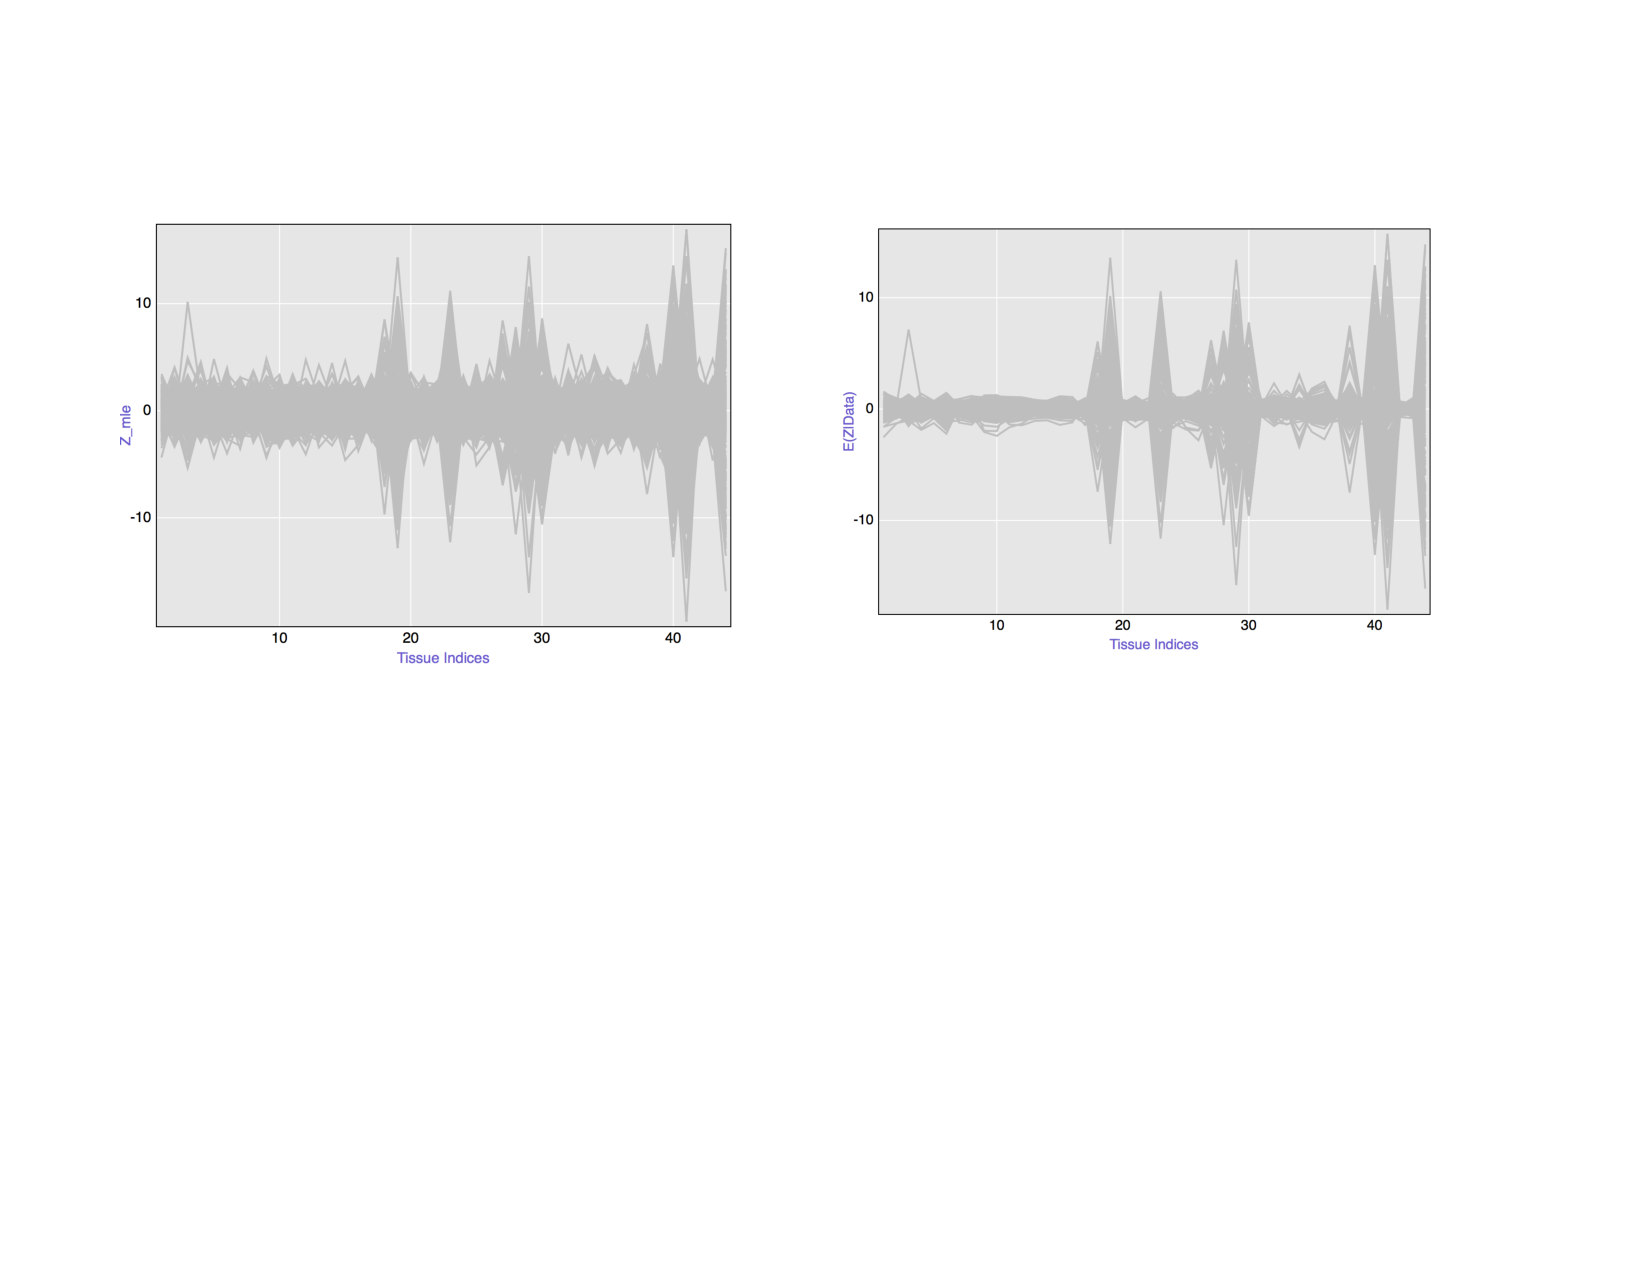
\includegraphics[width=8cm]{Figures/tspecsmooth.pdf}
\end{center}
\caption{\textbf{Tissue Specificity} At an LFSR threshold of 0.05, we can ask how many QTL are specific to a given tissue. Several patterns of tissue-specific QTLs stand out: transformed cell types, testis, thyroid, and whole blood. Tissue specific eQTL demonstrate the smoothing feature of this joint shrinkage approach}
\label{fig:tspec}
\end{figure}\newline




\subsection{Quantifying Heterogeneity}


Armed with a vector of effect size estimates across 44 tissues, $\bm{b_{j}}$, we can move beyond asking in how many tissues is a given gene-snp pair significant (Figure \ref{fig:het}), and ask about the relationship in effect size and direction among tissues in which the gene-snp pair is active.

%\textbf{Figure: Number of Tissues Significant}

\newline
\begin{figure}[htbp]
\includegraphics[width=10cm]{Figures/PlotsForPaper_files/figure-html/unnamed-chunk-18-1.png}\\
\includegraphics[width=10cm]{Figures/PlotsForPaper_files/figure-html/unnamed-chunk-23-1.png}\\
\caption{\textbf{Top: Number of Tissues Significant} At a given LFSR threshold (0.05), we can ask for each QTL, in how many tissues is it considered `significant'. However, armed with new information about effect size we can ask additional questions about heterogeneity, \textbf{Bottom: Heterogeneity in Magnitude:} For each gene-snp pair, we can ask how many tissues is the effect at least $50\%$ of the maximal effect. Above, we consider the distribution of this `Heterogeneity Index' with and without brains included in the analysis}
\label{fig:het}
\end{figure}\newline



From a biological standpoint, we might predict that effects of a different sign are rare. Considering this results with and without the inclusion of the brain tissues, which appear to behave as a strongly correlated group, we observe several phenomenon. The majority of gene-snp pairs are consistent in sign (indeed, only about $20\%$ of genes show two significant effects of a different sign when including brain, and even fewer $(14.8\%)$ when excluding brains, see Table \ref{table:het}) and removing brains from our analysis tends to push us towards consistency, suggesting that brain appears to behave as a large tissue-specific entity. After normalizing each gene-snp effect size coefficient $b_{jr}$ by the effect size with the maximum value for the gene, we can also ask what proportion of these are positive. We again recognize homogeneity with $83\%$ (all tissues) and $87\%$  (excluding brain) demonstrating positive normalized effects, respectively. \newline


%%\textbf{Figure: Sign Heterogeneity Distribution Figure}
%\newline
%\begin{figure}[htbp]
%\includegraphics[width=10cm]{Figures/PlotsForPaper_files/figure-html/unnamed-chunk-20-1.png}\\
%\caption{\textbf{Heterogeneity in Sign} For each gene-snp pair, we select the effect across tissues with the maximal absolute value and ask how many estimated effects possess a different sign. Homogenous SNPs in sign will thus be at the left of the distribution, while gene-snp pairs with many tissues different than the effect of largest (absolute) size will shift to the right}
%\label{fig:signhet}
%\end{figure}\newline

Furthermore, we can now quantify the heterogeneity index in magnitude described in the simulation framework above, and ask, for each gene, in how many tissues is the effect greater than equal to a significant fraction, here $50\%$ of the maximum effect (\ref{fig:het}). Genes binned in the left of this distribution are quantitatively specific because the effect is close to the maximal effect in few tissues, while homogenous genes be featured towards the right of the distribution (maximal value at 44) as the majority of their effects across tissues are similar in magnitude. Again, excluding brain from the analysis tends to nudge us towards a belief in consistency (Table \ref{table:het}).

Taken together, these results suggest the presence of consistency in sign in our data set, and a bimodal distribution of heterogeneity in magnitude.

\begin{table}[htbp]
\caption{Heterogeneity Comparison}
\centering
\begin{tabular}{c c c c}
\hline\hline
Data & All Tissues  & No Brains  \\ [0.5ex] % inserts table %heading
\hline
Consistent in Sign $E(b_{jrnorm}|D)$ $>$ 0) &0.833&0.880 \\
%E(DifferentSign (no threshold)&0.906 ( 0.87 no brains) &0.597&0.481\\
E(Consistent SignPosteriorMean$\mid$ LFSR$\leq$0.05)&0.802&0.852\\
E(At least 50\% max value) &0.354&0.449\\
%Sign Change &0&0.184&0.179\\[1ex]
\hline
\end{tabular}
\label{table:het}
\caption{\textbf{Heterogeneity Analysis} After normalizing each gene-snp-effect size coefficient by the effect size with maximal value at that gene ($b_{jr}$), we can ask how many of these gene-snp effect coefficients are positive. Similarly, at a given significance threshold, we can ask how many gene-pairs contain effects of different signs across tissues. At an arbitrary LFSR threshold of 0.05 for instance, we note that $80\%$ of genes are homogenous in sign when all tissues are considered. Excluding brains from our analysis, this rises to $85\%$. To evaluate consistency in magnitude, we can ask how many gene-snp-tissue effects are greater than $50\%$ of the maximal effect across tissues for the pair. Again, we see that excluding brains from our analysis tends to push this towards consistency.}
\end{table} \newline


%\textbf{Figure: Magnitude Heterogeneity Index Distribution}


Attempting to understand which genes tend to behave the most homogeneously or heterogeneously, we can plot (Figure \ref{fig:biplot}) the value used to normalize each gene, e.g., the `maximum' effect size across tissue of the gene, against the normalized values. We can see that if a large effect is present, it tends to be in the presence of homogenous effects across subgroups, while small normalizing effects tend to be in the presence of effects that are more variable in sign and magnitude. Furthermore, aggregating the gene-snp pairs at a given heterogeneity index and classifying them by the effect used to normalize (e.g., the `max effect') we can see that gene-snp pairs with greater Heterogeneity Indices tend to have larger effects on average, and the tissue-specific patterns again become more evident by plotting these QTL across tissues (Figure \ref{fig:biplot}, far right).
\begin{figure}[htbp]
%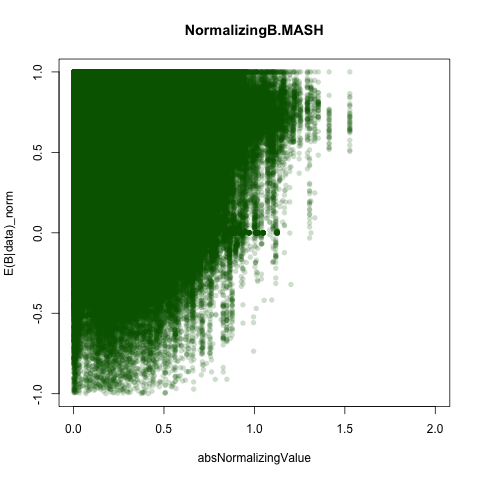
\includegraphics[width=5cm]{Figures/normstuffeb_nobrain.png}&
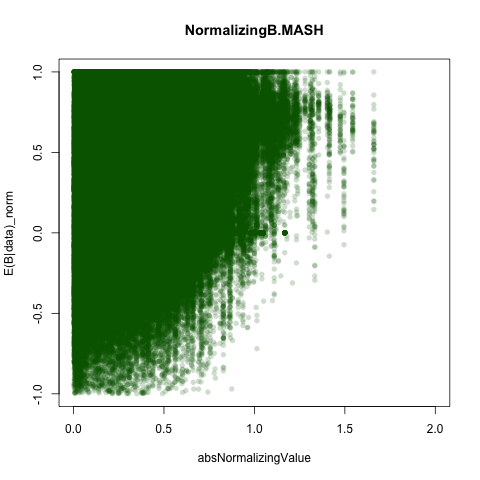
\includegraphics[width=5cm]{Figures/normstuffeb_alltissues.png}&
\includegraphics[width=5cm]{Figures/PlotsForPaper_files/figure-html/unnamed-chunk-24-1.png}\\
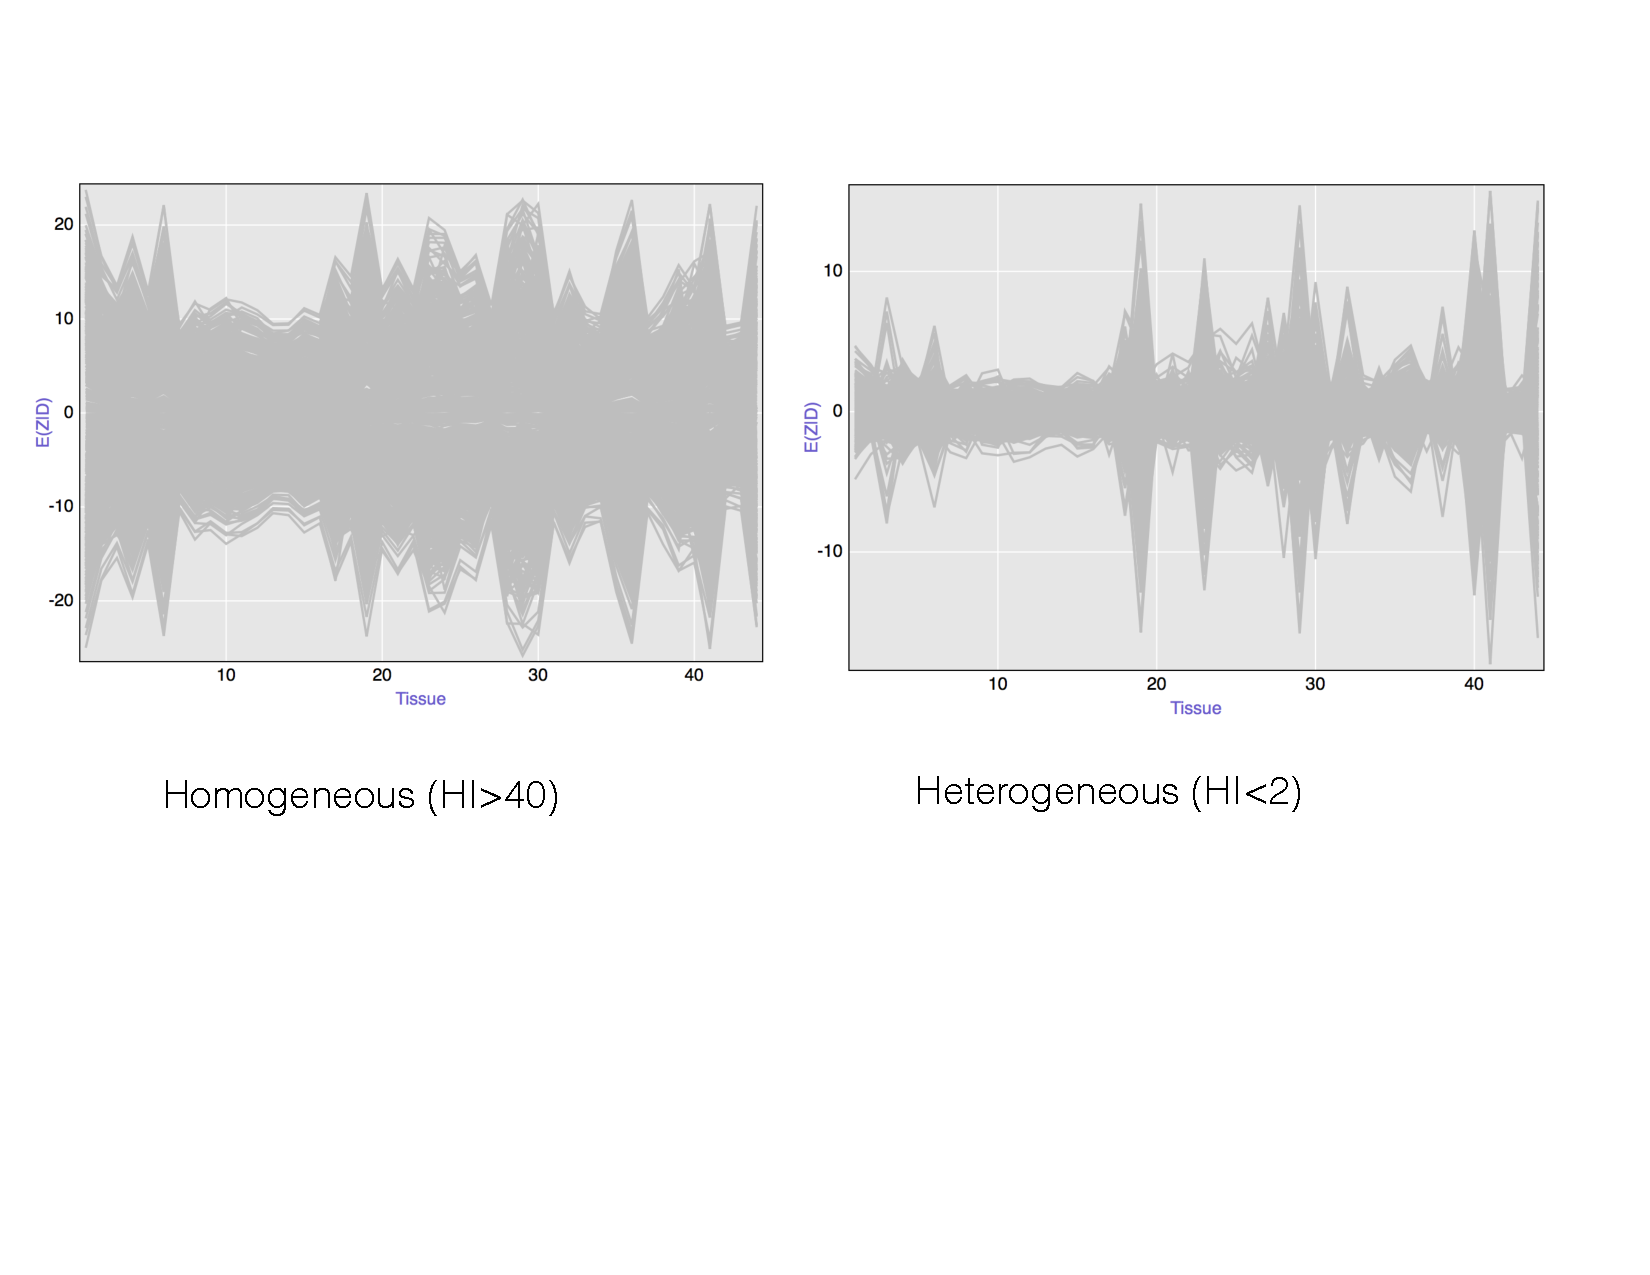
\includegraphics[width=10cm]{Figures/hetvshomqtl.pdf}
\caption{\textbf{Understanding Which Effects are the most homogenous} For each gene-snp pair, we plot the normalized gene-snp-tissue-effect (e.g., $b_{jr}$) against the largest absolute effect size for the genes. To learn which genes are more quantitatively homogeneous, we can see that eQTLs in which a large effect is present tend to have more consistent effects across the board, and thus occur in the presence of many normalize $b_{jr}$ close to 1. Furthermore, aggregating genes by their Heterogeneity Index and reporting the median maximal effect for genes of a given H class, we see that the maximum value tends to increase with homogeneity. We can segregate homogenous and heterogenous eQTL and consider their activity across tissues.}
\label{fig:biplot}
\end{figure}

%\textbf{Figure: QTL chart by HI index: homogenous or heterogenous}
%\textbf{Figure: Insert Plot of Normalized Effect vs Max value (e.g., biplot) and Median Max Effect By HI Index}




%In how many genes do there exists effects of a different sign? 
%9,597 (59.7%) vs 7,723 (48.1%)
% What about effects at a given significance threshold?
%3,180 with brain includes (19.8%), 2,377 no brain at an LFSR threshold of 0.05 ( 14.8%)
%Gene.snp.tissue.effects (i.e., b.j.r)
%With brains: Proportion b.j.r norm>0: 83.3 % Without brains: 88%
%Proportion b.j.r norm>50%: 35.4 vs 44.9%
